\documentclass[color=usenames,dvipsnames]{beamer}\usepackage[]{graphicx}\usepackage[]{color}
% maxwidth is the original width if it is less than linewidth
% otherwise use linewidth (to make sure the graphics do not exceed the margin)
\makeatletter
\def\maxwidth{ %
  \ifdim\Gin@nat@width>\linewidth
    \linewidth
  \else
    \Gin@nat@width
  \fi
}
\makeatother

\definecolor{fgcolor}{rgb}{0.345, 0.345, 0.345}
\newcommand{\hlnum}[1]{\textcolor[rgb]{0.686,0.059,0.569}{#1}}%
\newcommand{\hlstr}[1]{\textcolor[rgb]{0.192,0.494,0.8}{#1}}%
\newcommand{\hlcom}[1]{\textcolor[rgb]{0.678,0.584,0.686}{\textit{#1}}}%
\newcommand{\hlopt}[1]{\textcolor[rgb]{0,0,0}{#1}}%
\newcommand{\hlstd}[1]{\textcolor[rgb]{0.345,0.345,0.345}{#1}}%
\newcommand{\hlkwa}[1]{\textcolor[rgb]{0.161,0.373,0.58}{\textbf{#1}}}%
\newcommand{\hlkwb}[1]{\textcolor[rgb]{0.69,0.353,0.396}{#1}}%
\newcommand{\hlkwc}[1]{\textcolor[rgb]{0.333,0.667,0.333}{#1}}%
\newcommand{\hlkwd}[1]{\textcolor[rgb]{0.737,0.353,0.396}{\textbf{#1}}}%
\let\hlipl\hlkwb

\usepackage{framed}
\makeatletter
\newenvironment{kframe}{%
 \def\at@end@of@kframe{}%
 \ifinner\ifhmode%
  \def\at@end@of@kframe{\end{minipage}}%
  \begin{minipage}{\columnwidth}%
 \fi\fi%
 \def\FrameCommand##1{\hskip\@totalleftmargin \hskip-\fboxsep
 \colorbox{shadecolor}{##1}\hskip-\fboxsep
     % There is no \\@totalrightmargin, so:
     \hskip-\linewidth \hskip-\@totalleftmargin \hskip\columnwidth}%
 \MakeFramed {\advance\hsize-\width
   \@totalleftmargin\z@ \linewidth\hsize
   \@setminipage}}%
 {\par\unskip\endMakeFramed%
 \at@end@of@kframe}
\makeatother

\definecolor{shadecolor}{rgb}{.97, .97, .97}
\definecolor{messagecolor}{rgb}{0, 0, 0}
\definecolor{warningcolor}{rgb}{1, 0, 1}
\definecolor{errorcolor}{rgb}{1, 0, 0}
\newenvironment{knitrout}{}{} % an empty environment to be redefined in TeX

\usepackage{alltt}
%\documentclass[color=usenames,dvipsnames,handout]{beamer}

%%\usepackage[roman]{../pres1}
\usepackage[sans]{../pres1}
\usepackage{graphicx}
\usepackage{bm}

%\usepackage{Sweave}




\IfFileExists{upquote.sty}{\usepackage{upquote}}{}
\begin{document}




\begin{frame}[plain,fragile]
  \centering
    \huge
    The BIDE model \\
    \large
    January 14, 2019 \\
    \vfill

\begin{columns}
  \column{\dimexpr\paperwidth-10pt}
  \centering
  \includegraphics[width=0.75\textwidth]{figure/bide0-1} \\
\end{columns}
\end{frame}



\section{Definitions}


\begin{frame}
  \frametitle{Today's topics}
  \LARGE
  \only<1>{\tableofcontents}%[hideallsubsections]}
\end{frame}


\begin{frame}
  \frametitle{Definitions}
%  \begin{block}{Population dynamics}
  {\bf Population dynamics \\}
    The study of spatial and temporal variation in population size and structure
%  \end{block}
  \pause
  \vfill
%  \begin{block}{Population}
  {\bf Population \\}
    Individuals of the same species occuring in the same geographic region
%  \end{block}
  \pause
  \vfill
%  \begin{block}{Population size and structure}
  {\bf Population size and structure \\}
    {\color{Red}
%      \bf
      \it Size:} Abundance \\
    {\color{Red}
%      \bf
      \it Structure:} Distribution of individuals among age groups, sexes,
    habitat patches, etc\dots
%  \end{block}
\end{frame}



\section{Modeling 101}






% \begin{frame}
%   \frametitle{What is a model?}
%   \Large
%   \pause
%   A model is an abstraction of reality. \par
%   \pause
%   \vfill
% %  By definition all models are wrong. \par
% %  \pause
% %  \vfill
% %  \includegraphics[width=0.8\textwidth]{figs/Box-quote}
%   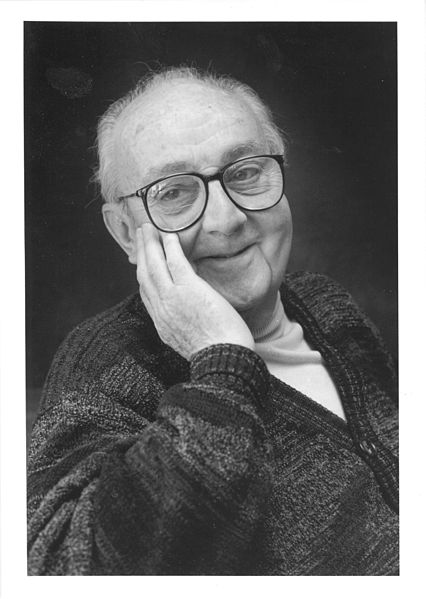
\includegraphics[width=0.2\textwidth]{figs/Box}
%   ``All models are wrong, but some are useful.'' G.E.P. Box (1987)
% \end{frame}



\begin{frame}
  \frametitle{Models and science}
%  Applied Ecology and the need for objectivity in obtaining reliable
%  knowledge
  \Large
%  \pause
  A model is an abstraction of reality. \par
  \pause
  \vfill
  \Large
  {\bf Models help us\dots}
  \begin{itemize}[<+->]
    \item Describe complex natural systems in a manageable way
    \item Predict future outcomes
    \item Cope with uncertainty %, specifically random
%      variation and imperfect knowledge
    \item Formalize hypotheses
    \item Evaluate hypotheses by comparing predictions with observations
  \end{itemize}
\end{frame}




\begin{frame}
  \frametitle{But don't models require assumptions?}
  \large
  \pause
  Yes. %\pause So what?
  \pause
  \vfill
  We have to simplify, so we have to make assumptions.
  \pause
  \vfill
  We do this all the time.
  \pause
  \vfill
  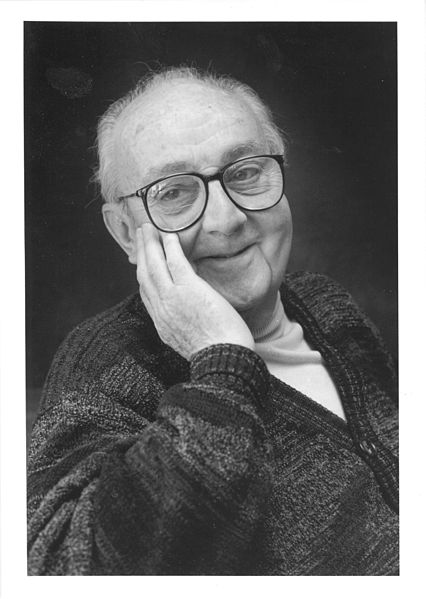
\includegraphics[width=0.2\textwidth]{figs/Box}
  ``All models are wrong, but some are useful.'' G.E.P. Box (1987)
\end{frame}




\begin{frame}
  \frametitle{Model validation}
  \Large
  {\bf Putting the model to the test}
  \begin{itemize}[<+->]
    \item How well does it predict?
    \item Will your results hold up in court?
    \item Can your results be replicated/reproduced?
  \end{itemize}
\end{frame}








%\section{Modeling 101}




\begin{frame}
  \frametitle{Types of models}
  \LARGE
  \begin{itemize}
    \item {\color<2>{Red} Conceptual}
    \item Physical
    \item Graphical
%    \item {\color<2>[rgb]{0,0,1} Mathematical}
    \item {\color<2>{Red} Mathematical}
    \item {\color<2>{Red} Statistical}
  \end{itemize}
\end{frame}





\section{BIDE}


\begin{frame}
  \frametitle{The BIDE model}
  \huge
  \[
  N_{t+1} = N_t + B_t + I_t - D_t - E_t
  \]
  \large
  \vfill
%  \centering where \flushleft \par
  \centering \rule{4cm}{1pt} \flushleft \par
  \vfill
  \Large
  $N_t$: population size (state variable) at time $t$ \\
  $B_t$: births \\
  $I_t$: immigrants \\
  $D_t$: deaths \\
  $E_t$: emigrants
  \note{Notation... differs from }
  \note{These are not rates}
  \note{Implies several things. Area must be well-defined. Time must
    be discrete, as opposed to continuous}
  \note{Ask students to write a factor that could influence each parameter}
  \note{Classify each variable: attributes of the animal, other biotic
    factors e.g. competitors/prey, attributes of the habitat, and population}
  \note{Represent BIDE models as a conceptual model}
  \note{Could you get data on each of these variables?}
\end{frame}


\begin{frame}
  \frametitle{The BIDE model}
  \huge
  \[
  N_{t+1} = N_t + B_t + I_t - D_t - E_t
  \]
  \large
  \vfill
  {\bf As written, this model implies the following:}
  \begin{itemize}%[<+->]
    \item<1-> $B$, $I$, $D$, and $E$ are not rates, they
      are the number of events at time $t$.
    \item The model is {\bf deterministic}, not {\bf stochastic}
    \item Time is discrete, not continuous
%    \item Space is well-defined
  \end{itemize}
  \vspace{0.5cm}
  \pause
  \bf In reality, things are more complicated, and interest lies in
  understanding the factors influencing each process.\par
%    \pause
%    \vspace{0.5cm}
%    \centering
%    {\color{blue}
%    QUESTION:} What influences these processes? \\
  \note{Spend the rest of lecture doing a group exercise to create
    list of factors influencing each process?}
\end{frame}



\section{Assignment}


\begin{frame}
  \frametitle{Assignment}
  \Large
  \bf
  Read the first 3 pages of Chapter 3 in Conroy and Carroll \\
%
%  \vfill
%  Expect a quiz on Monday
\end{frame}







\end{document}
